%----------------------------------------------------------------------------------------
%	SECTION 1.1
%----------------------------------------------------------------------------------------

\section{Espacios M\'etricos.}

\begin{definition}
    Una \textbf{M\'etrica} sobre un conjunto $X$ es ina funcion  $d:X \times X \rightarrown \R$ tal
    que para toda $x,yz \in X$:
        \begin{enumerate}[label=(\arabic*)]
            \item $d(x,y) \geq 0$ y $d(x,y)=0$ si y solo si $x=y$.

            \item $d(x,y)=d(y,x)$.

            \item $d(x,z) \leq d(x,y)+d(y,z)$ (La Desigualdad Triangular).
        \end{enumerate}
        Si $d$ es una m\'etrica sobre el conjunto $X$, entonces decimos que el par ordenado  $(X,d)$
        es un \textbf{espacio m\'etrico}, y que $ d(x,y)$ es la \textbf{distancia} entre $x$ y y.
\end{definition}

\begin{example}
    Sea $X=\R$ y  $d=|\cdot|$, entonces $(\R,|\cdot|)$ es una espacio m\'etrico. Para $X=\R^2$ y
    $d=||\cdot||$,  $(\R^2,||\cdot||)$ tambien es un espacio metrico.		
\end{example} 

\begin{example}[La M\'etrica Discreta]
    Sea $X$ cualquier conjunto, y sea  $d(x,y)=\begin{cases} 1 & x \neq y \\ 0 & x=y \\\end{cases}$ 
    Vemos que las propiedades $(1)$ y $(2)$ estan satisfecho. Tambien vemos que para $x,y,z \in X$
    que  $d(x,z)=1,0$ y que $d(x,y),d(y,x)=1,0$. Pues $d(x,y)+d(y,z)=2,1,0$, pues en todo caso
    $d(x,z) \leq d(x,y)+d(y,z)$. $(X,d)$ es un espacio metrico.
\end{example} 

\begin{definition}
    Sea $(X,d)$ un espacio m\'etrico, $x \in X$ y  $\epsilon>0$. Definimos el conjunto
    $B_d(x,\epsilon)=\{y \in X: d(x,y)<\epsilon\}$ como la \textbf{$\epsilon$-bola con centro en
    $x$}. Tambien es conocido como la \textbf{bola abierta centrado en $x$ de radio  $\epsilon$}.
\end{definition}

\begin{example}
    \begin{enumerate}[label=(\arabic*)]
        \item Sea $X=\{a,b,c\}$ y sea $d$ la metrica disscreta. Entonces  $B_d(a,\frac{1}{2})=\{a\}$, 
        $B_d(a,4)=X$ y $B_d(a,1)=\{a\}$.

    \item Sea $X=\R^n$ y defina  $d:\R^n \times \R^n \rightarrow \R$ talque
        $d(x,y)=\sqrt{\sum{(x_i-y_i)^2}}=||x-y||$. Claramente los primeros $2$ propiedades se
        satisfechan. Ahora por la desigualdad de Cauchy-Schwarz, tenemos que  $|\vbrack{x,y}| \leq
        ||x||||y||$ y por la desigualdad de Minowski, tenemos que $||x+y|| \leq ||x||+||y||$. Puse
        usando estos dos desigualdades vemos que  $d$ es un m\'etrico. Llamamos a este m\'etrico el
        \textbf{m\'etric Euclideano} y lo denotaremos como $||\cdot||$.

        Tambien existen otros m\'etricos en  $\R^n$. Definimos la \textbf{m\'etrica taxista} como
        $d(x,y)=\sum{|x_i-y_i|}$ y la \textbf{m\'etrica cuadrada} como $\rho(x,y)=\max{|x_1-y_1|,
        \dots, |x_n-y_n|}$. Aqui vemos que pa los puntos $x=(2,3)$ y $y=(6,6)$ en $X=\R^2$ que
        $||x-y||=\sqrt{(2-6)^2+(3-6)^2}=5$, $d(x,y)=|2-6|+|3-6|=7$ y que
        $\rho(x,y)=\max{|2-6|,|3-6|}=4$; y tenemos que $B_{||\cot||}(0,1)=\{x \in \R^2:
        ||x||<1\}=\{x \in \R^2: \sqrt{x_1^2+x_2^2}<1\}$, que $B_d(0,1)=\{x \in \R^2: d(x,0)<1\}=\{x
    \in\R^2: |x_1|+|x_2|<1\}$ y que $B_{\rho}(0,1)=\{x \in \R^2:\rho(x,0)<1\}=\{x \in \R^2:
\max{|x_1|,|x_2|}<1\}$
    \end{enumerate} 		
\end{example} 

\begin{figure} 
    \centering
    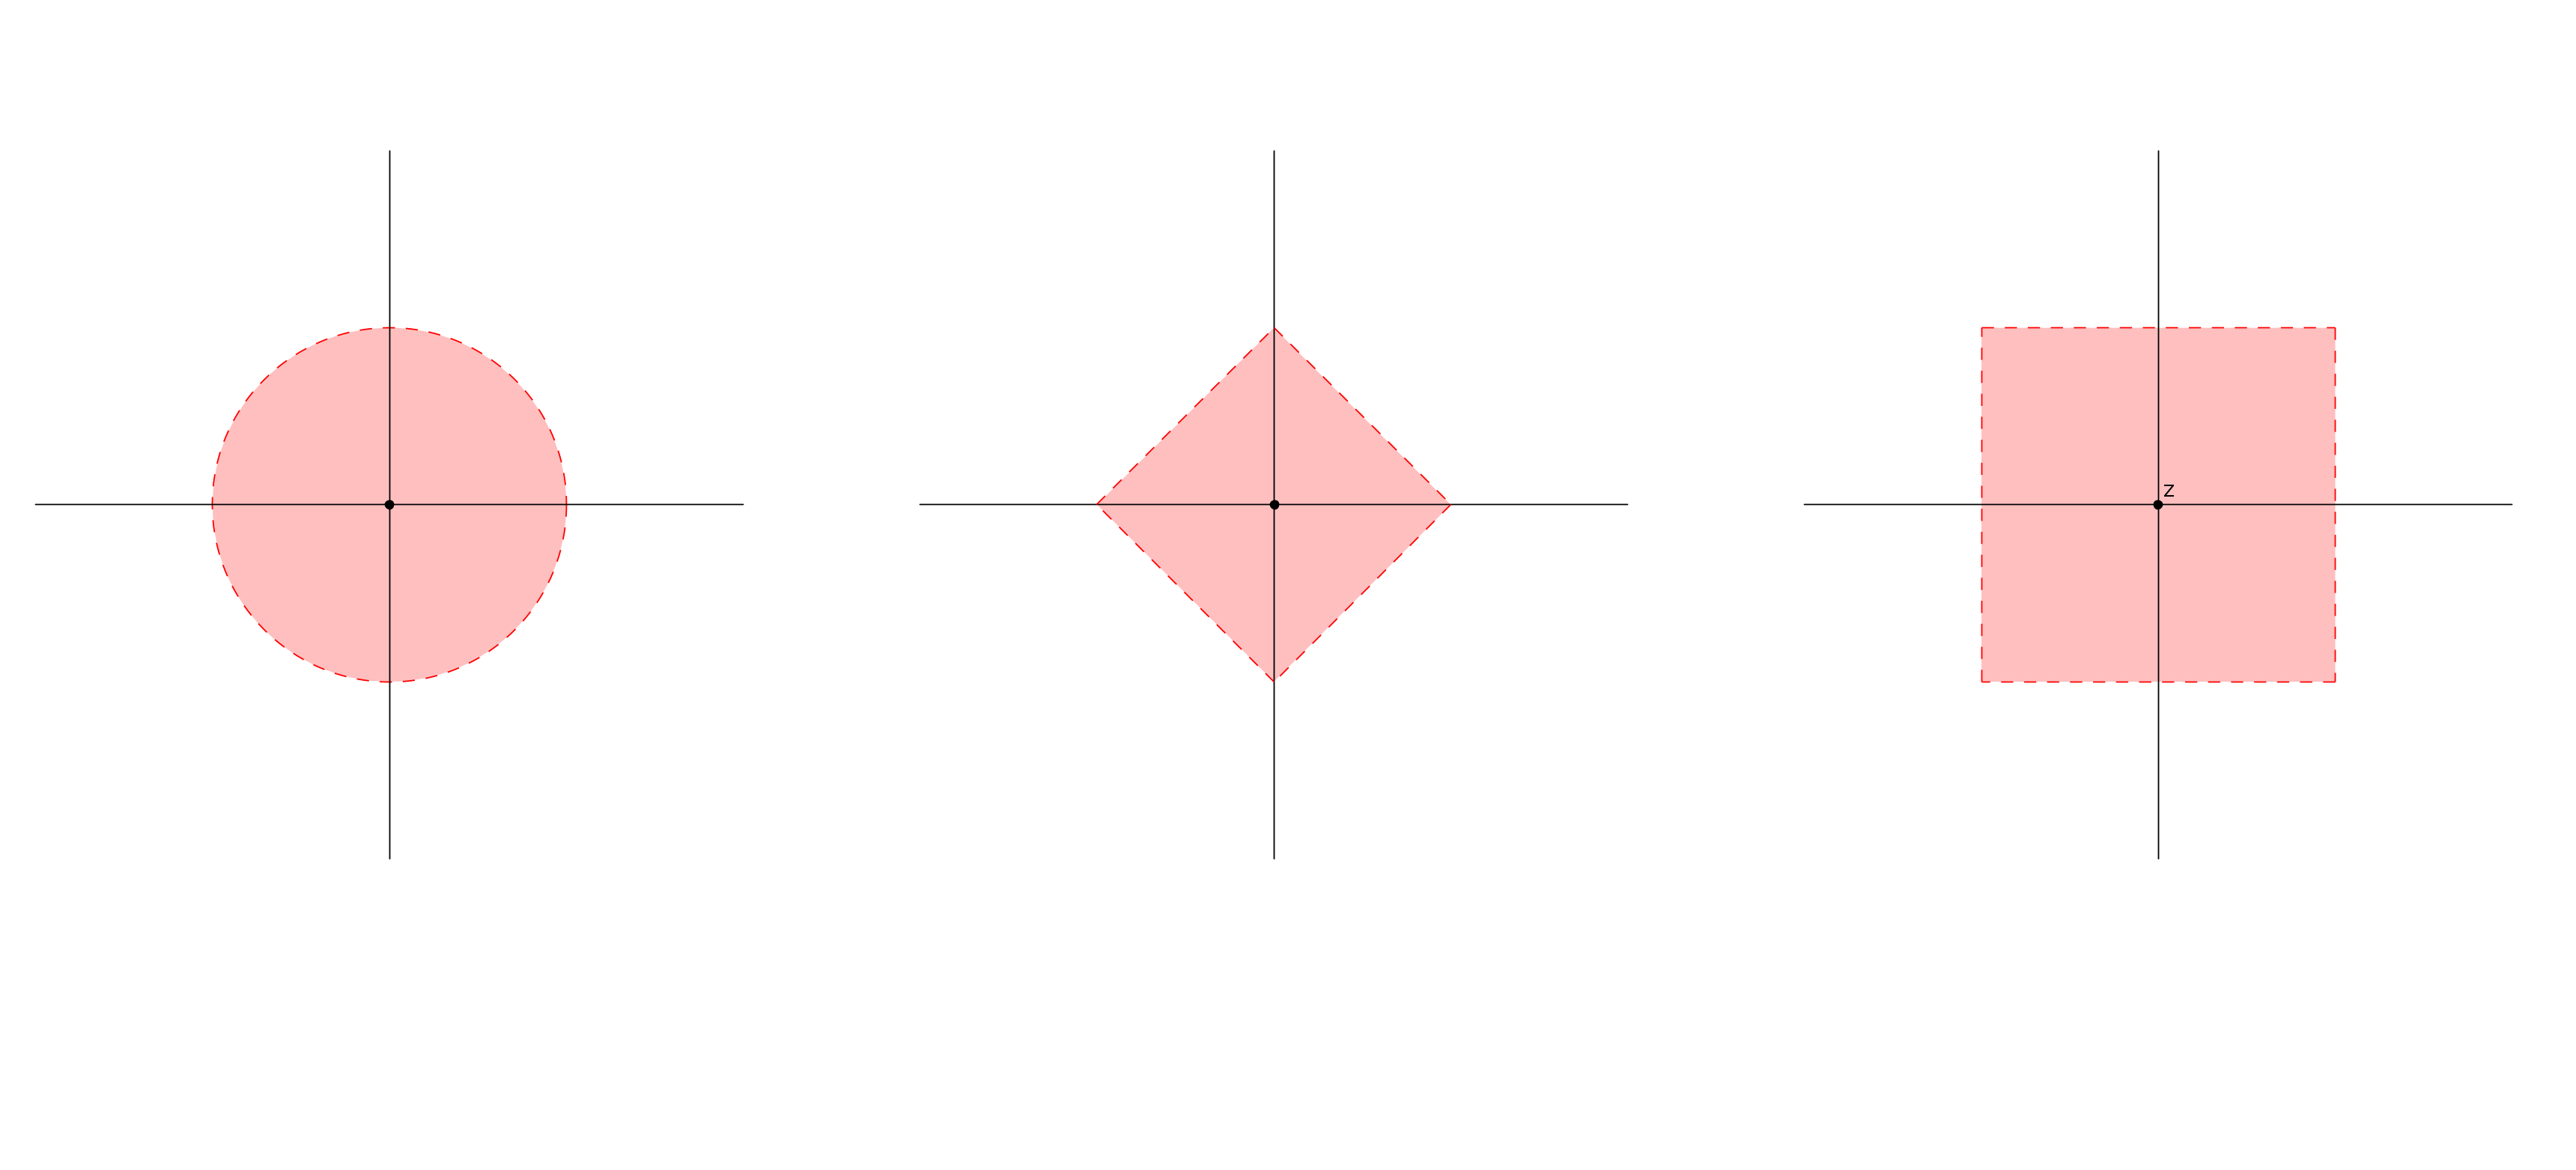
\includegraphics[scale=0.4]{Figures/Chapter1/euclideanTaxicabSquare.png}
    \caption{El m\'etrico Euclideano, el m\'etrico taxista, y el m\'etrico cuadrado.}
    \label{fig_1.1}
\end{figure}

\begin{definition}
    Sean $(X,d)$ y $(Y, \rho)$ espacios metricos. Una funci\'on $f:X \rightarrow Y$ es
    \textbf{continua en el punto $a \in X$} si para cade $\epsilon>0$ existe un  $\delta>0$ tal que
    s\'i  $x \in X$ y  $d(a,x)<\delta$, entonces $\rho(f(a),f(x))<\epsilon$. Decimos que $f$ es
    \textbf{continua} si es continua en casa punto de $X$.
\end{definition}

\begin{example}
    Sean $(X,d)$ y $(Y,\rho)$ espacios m\'etricos y sea $ y_0 \in Y$ y defina $i:X \rightarrow X$
    for  $x \rightarrow x$ y  $c:X \rightarrow Y$ por $x \rightarrow y_0$. Para $i$, sea
    $\epsilon>0$ y coge  $\delta=\epsilon$. Pues vemos que  $d(a,x)=d(i(a),i(x))<\delta=\epsilon$.
    Pues $i$ es continua en todo  $X$. Ahora sea  $\epsilon>0$ y  $\delta>0$, tenemos qque
    $d(a,x)<\delta$ implica que $\rho(c(x),c(a))=\rho(y_0,y_0)=0<\epsilon$ pues $c$ tambien es
    continua en  $X$.
\end{example}

\begin{theorem}\label{1.1.1}
    Sean $(X,d)$ y $(Y,\rho)$ espacios m\'etricos, entonces $f:X \rightarrow Y$ es continua en el
    punto $a \in X$ si y solo si para cada bola abierta  $B_{\rho}(f(a),\epsilon)$, existe una bola
    abierta $B_d(a,\delta)$ tal que $f(B_d(a,\delta)) \subseteq B_{\rho}(f(a),\epsilon)$.
\end{theorem}
\begin{proof}
    Sea $f$ continua en  $a$, entonces dado  $\epsilon>0$ considere la bola
    $B_{\rho}(f(a),\epsilon)$, pues existe un $\delta>0$ tal que si  $x \in X$ y  $d(a,x)<\delta$,
    entonces $\rho(f(a),f(x))<\epsilon$. Pues vemos que como $x \in B_d(a,\delta)$, tenemos que
    $f(B_d(a,\delta)) \subseteq B_{\rho}(f(a),\epsilon)$

    Ahora suponga que para cada $B_{\rho}(f(a),\epsilon)$ hay un  $B_d(x,\delta)$ tal que
    $f(B_d(a,\delta)) \subseteq B_{\rho}(f(a),\epsilon)$. Entonces sea $x \in X$ con
    $d(x,a)<\delta$, entonces tenemos que $x \in B_d(a,\delta)$, pues por h\'ipotesis, $f(x) \in
    B_{\rho}(f(a),\epsilon)$, es decir que $\rho(f(x),f(a))<\epsilon$; por lo tanto $f$ es continua
    en  $a$.
\end{proof}
